\section{Content Delivery Network Characterization by Distributed Active Measurements}\label{sec:aslevel:crowd}

%The most popular peer-to-peer overlay network today is BitTorrent.
%Therefore we focus on BitTorrent.
% motivation
%Internet video constitutes more than half of all consumer Internet traffic globally, and its percentage will further increase \cite{ciscovni2013}. Most of the video traffic is delivered by content delivery networks (CDNs). Today the world's largest video CDN is YouTube. Since Google took over YouTube in 2006 the infrastructure of the video delivery platform has grown to be a global content delivery network.
%The global expansion of the CDN was also necessary to cope with growing demand of user demands and the high expectations on the video playback. Therefore, content delivery networks try to bring content geographically close to users.
%However, the traffic from content delivery networks is highly asymmetric and produces a large amount of costly inter-domain traffic \cite{labovitz2010internet}. Especially Internet Service Providers~(ISPs) providing access to many end users have problems to deal with the huge amount of traffic originating from YouTube. Furthermore, the Google CDN is constantly growing and changing, which makes it difficult for access providers to adapt their infrastructure accordingly.

% problem statement
%To understand and monitor the impact of YouTube traffic on ISPs and the topology of CDNs appropriate measurements are acquired.
Today the world's largest video CDN is YouTube.
Since Google took over YouTube in 2006 the infrastructure of the video delivery platform has grown to be a global CDN.
By measuring its characteristics, conclusions can be drawn in order to develop traffic management mechanisms that handle the huge amount of traffic the YouTube CDN puts on access networks.
Due to YouTube's load-balancing and caching mechanisms the YouTube video server selection is highly dependent on the location of the measurement points.
Hence, we need a globally distributed measurement platform to perform active measurements to uncover the location of YouTube servers.
%Recent work \cite{adhikari2012vivisecting,adhikari2011you} has performed such measurements in PlanetLab~\cite{planetlab}, a global test bed that provides measurement nodes at universities and research institutes.
The problem is that probes disseminated from PlanetLab nodes origin solely from National Research and Education Networks~(NRENs). This may not reflect the perspective of access ISPs which have a different connection to the YouTube CDN with different peering or transit agreements.
% our methodology
To achieve a better view on the YouTube CDN from the perspective of end users in access networks, we use a commercial crowdsourcing platform to recruit regular Internet users as measurement probes.
This complementary view can help to gain a better understanding of the characteristics of Video CDNs.
%Thus, we increase the coverage of vantage points for the distributed measurement of the YouTube CDN.
To evaluate the impact of the measurement platform and the coverage of their vantage point, we perform the same measurements using PlanetLab nodes and crowdsourcing users and compare the obtained results.

% our contribution
%Our measurements show that distributed measurements in PlanetLab are not capable to capture a globally distributed network, since the PlanetLab nodes are located in NRENs where the view on the Internet is limited. We demonstrate that recruiting users via crowdsourcing platforms as measurement probes can offer a complementary view on the Internet, since they provide access to real end users devices located out side of these dedicated research networks.
%Concepts like ALTO or economic traffic management (ETM) \cite{hossfialong} need a global view of the CDN structure to optimize traffic beyond the borders of ISPs.
%what in turn  might have implications for network operators in mechanism design and resource provisioning.
%Finally, models for simulation and performance evaluation of mechanisms incorporating CDNs need to apply the characteristics identified by crowd sourced network measurements.
%In this work, we propose a new measurement methodology which benefits of the distribution of crowdsourcing workers on internet access provider networks.

% structure
The measurements conducted in the PlanetLab and via crowdsourcing are described in Section~\ref{sec:crowd:method}.
In Section~\ref{sec:crowd:results} we provide details on the measurement results and their importance for the design of distributed network measurements.

%% todo matthias
test

\subsection{Distributed Active Measurement Setup}
\label{sec:crowd:method}

To assess the capability of crowdsourcing for distributed active measurements we conduct measurements with both  PlanetLab and the commercial crowdsourcing platform Microworkers~\cite{microworkers}.
We measure the global expansion of the YouTube CDN by resolving physical server IP addresses for clients in different locations.

\subsubsection{Description of the PlanetLab Measurement}

PlanetLab is a publicly available test bed, which currently consists of 1173 nodes at 561 sites.
The sites are usually located at universities or research institutes.
Hence, they are connected to the Internet via NRENs.
To conduct a measurement in PlanetLab a slice has to be set up which consists of a set of virtual machines running on different nodes in the PlanetLab test bed.
Researchers can then access these slides to install measurement scripts.
In our case the measurement script implemented in Java extracted the server hostnames of the page of three predetermined YouTube videos and resolved the IP addresses of the physical video servers.
The IP addresses of the PlanetLab clients and the resolved IP addresses of the physical video servers were stored in a database.
To be able to investigate locality in the YouTube CDN, the geo-location of servers and clients is necessary.
For that purpose the IP addresses were mapped to geographic coordinates with MaxMinds GeoIP database \cite{geolite}.
The measurement was conducted on 220 randomly chosen PlanetLab nodes in March 2012.

\subsubsection{Description of the Crowdsourcing Measurement}
To measure the topology of the YouTube CDN from an end users point of view who is connected by an ISP network we used the crowdsourcing platform Microworker~\cite{microworkers}.
The workers were asked to access a web page with an embedded Java application, which automatically conducts client side measurements.
These include, among others, the extraction of the default and fallback server URLs from three predetermined YouTube video pages.
The extracted URLs were resolved to the physical IP address of the video servers locally on the clients.
The IP addresses of video servers and of the workers client were sent to a server which collected all measurements and stored them in a database.

In a first measurement run, in December 2011, 60 different users of Microworkers participated in the measurements.
Previous evaluation have shown, that the majority of the platform users is located in Asia~\cite{conf2011-410}, and accordingly most of the participants of there first campaign were from Bangladesh.
In order to obtain wide measurement coverage the number of Asian workers participating in a second measurement campaign, conducted in March 2012, was restricted.
In total, 247 workers from 32 different countries finished the measurements successfully, identifying 1592 unique physical YouTube server IP addresses.

\subsection{Measurement Results and Their Implications}
\label{sec:crowd:results}

In this section we show the results of the distributed measurement of the global CDN.
The obtained results show the distribution of clients and servers over different countries.
Using a crowdsourcing platform, we derive accurate models for the distribution of cache servers on ASs, which are required for the performance evaluation and optimization of CDNs.
Furthermore, the mapping on autonomous systems gives insights to the coverage of the Internet.

\subsubsection{Distribution of Vantage Points on Countries}

To investigate the coverage of measurement points we study the distribution of the PlanetLab nodes and Crowdsourcing workers.
Figure~\ref{fig:PLSrc} shows the distribution of PlanetLab nodes on countries over the world.
The pie chart is denoted with the country codes and the percentage of PlanetLab nodes in the respective country.
Most of the 220 clients are located in the US with 15\% of all clients.
However, more than 50\% of the clients are located in West Europe.
Only few clients are located in different parts of the world.
The tailored distribution towards western countries is caused by the fact, that the majority of the PlanetLab nodes are located in the US or in West Europe.

\begin{figure}[bt]
    \centering
	\begin{subfigure}[t]{0.49\textwidth}
	\includegraphics[width=\textwidth]{aslevel/crowd/figs/PLSrc.pdf}
\caption{PlanetLab}
\label{fig:PLSrc}
\end{subfigure}
\begin{subfigure}[t]{0.49\textwidth}
	\includegraphics[width=\textwidth]{aslevel/crowd/figs/MWSrc.pdf}
\caption{Crowdsourcing}
 	\label{fig:MWSrc}
\end{subfigure}
    \caption{Distribution of measurement points on countries in a) PlanetLab and b) Crowdsourcing platform.}
    \label{fig:Src}
\end{figure}

%\begin{figure}[tb]
%	\centering
% 	\includegraphics[width=0.5\textwidth]{figures/Diagramme/Geo/PLSrc.pdf}
%  	\caption{Distribution of PlanetLab nodes over countries.}
%  	\label{fig:PLSrc}
%\end{figure}

Figure~\ref{fig:MWSrc} shows the geo-location of workers on the crowdsourcing platform.
In contrast to PlanetLab, most of the 247 measurement points are located in Asia-Pacific and East-Europe.
The majority of the participating workers 20\% are from Bangladesh (BD) followed by Romania (RO) and the US with 10\%.
This bias is caused by the overall worker distribution on the platform~\cite{conf2011-410}. However, this can be influenced to a certain extend by limiting the access to the tasks to certain geographical regions.
%The payment for crowdsourcing tasks is equal for all countries.
%Hence, the reward is higher for people living in developing countries with less value of money.
%This makes crowdsourcing platforms interesting for people in these countries and leads to a tailored distribution of clients towards different parts of the world.

%\begin{figure}[tb]
%	\centering
% 	\includegraphics[width=0.5\textwidth]{figures/Diagramme/Geo/MWSrc.pdf}
%  	\caption{Distribution of microworkers over countries.}
%  	\label{fig:MWSrc}
%\end{figure}
\subsubsection{Distribution of Identified YouTube Servers on Countries}

To investigate the expansion of the YouTube CDN we study the distribution of YouTube servers over the world.
Figure~\ref{fig:PLDst} shows the location of the servers identified by the PlanetLab nodes.
The requests are mainly directed to servers in the US. Only 20\% of the requests were directed to servers not located in the US.

\begin{figure}[bt]
    \centering
	\begin{subfigure}[t]{0.49\textwidth}
	\includegraphics[width=\textwidth]{aslevel/crowd/figs/PLDest.pdf}
  \caption{PlanetLab}
	\label{fig:PLDst}
  \end{subfigure}
	\begin{subfigure}[t]{0.49\textwidth}
	\includegraphics[width=\textwidth]{aslevel/crowd/figs/MWDest.pdf}
  \caption{Crowdsourcing}
 	\label{fig:MWDst}
  \end{subfigure}
    \caption{Distribution of physical YouTube servers on countries accessed from a) PlanetLab nodes and b) workers of a crowdsourcing platform.}
    \label{fig:Dst}
\end{figure}

%\begin{figure}[tb]
%	\centering
% 	\includegraphics[width=0.5\textwidth]{figures/Diagramme/Geo/PLDest.pdf}
%  	\caption{Distribution of YouTube servers accessed from PlanetLab nodes.}
%  	\label{fig:PLDst}
%\end{figure}

The servers identified by the crowdsourcing measurement are shown in Figure~\ref{fig:MWDst}.
The amount of requests being directed to servers located in the US is still high.
44\% of clients were directed to the US.
However, in this case the amount of requests resolved to servers outside the US is higher.
In contrast to the PlanetLab measurement many requests are served  locally in the countries of clients.
Furthermore, the decrease of 80\% to 44\% of request being directed to the US shows a huge difference.

%\begin{figure}[tb]
%	\centering
% 	\includegraphics[width=0.5\textwidth]{figures/Diagramme/Geo/MWDest.pdf}
%  	\caption{Distribution of YouTube servers accessed from crowdsourcing users.}
%  	\label{fig:MWDst}
%\end{figure}

Hence, network probes being overrepresented in the US and Europe leads to a limited  view of the content delivery network and the Internet.
This shows the impact of different locations of measurement points on the view of the CDN.
It also demands a careful choice of vantage points for a proper design of experiments in distributed network measurements.
Although both sets of measurement points are globally distributed the fraction of the CDN which is discovered by the probes has very different characteristics.

The amount of servers which is located in the US almost doubles for the PlanetLab measurement.
While 44\% of the requests are resolved to US servers in the Crowdsourcing measurement, nearly all requests of PlanetLab nodes are served by YouTube servers located in the US.
Although less than 15\% of clients are in US, requests are frequently directed to servers in the US. That means that there is still potential to further distribute the content in the CDN.

\subsubsection{Coverage of Autonomous Systems with YouTube Servers}

To identify the distribution of clients on ISPs  and to investigate the expansion of CDNs on autonomous systems we map the measurement points to the corresponding autonomous systems.

%\begin{figure}[tb]
%	\centering
% 	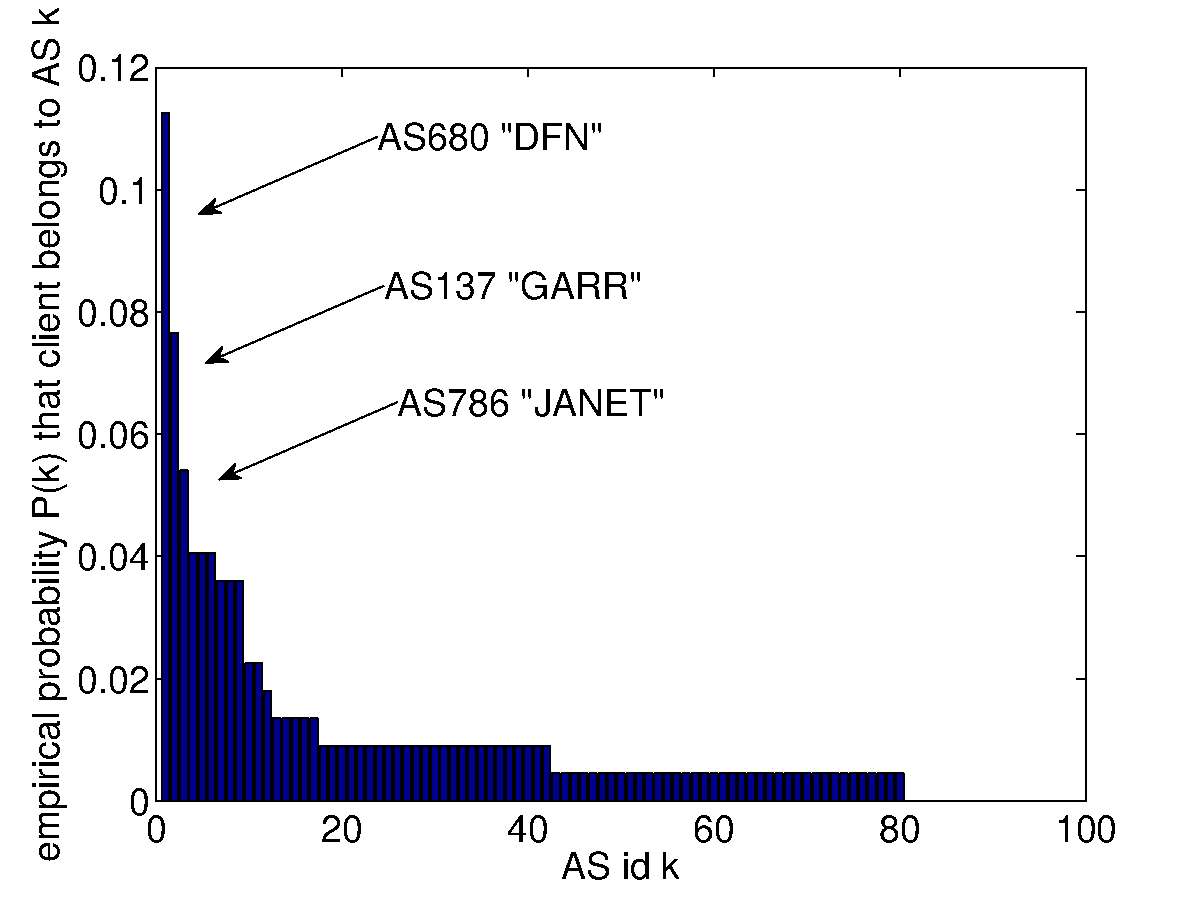
\includegraphics[width=0.5\textwidth]{figures/valli_AS_pl_src.pdf}
%  	\caption{Distribution of PlanetLab nodes over autonomous systems.}
%  	\label{fig:AS_mw_src}
%\end{figure}
%
%\begin{figure}[tb]
%	\centering
% 	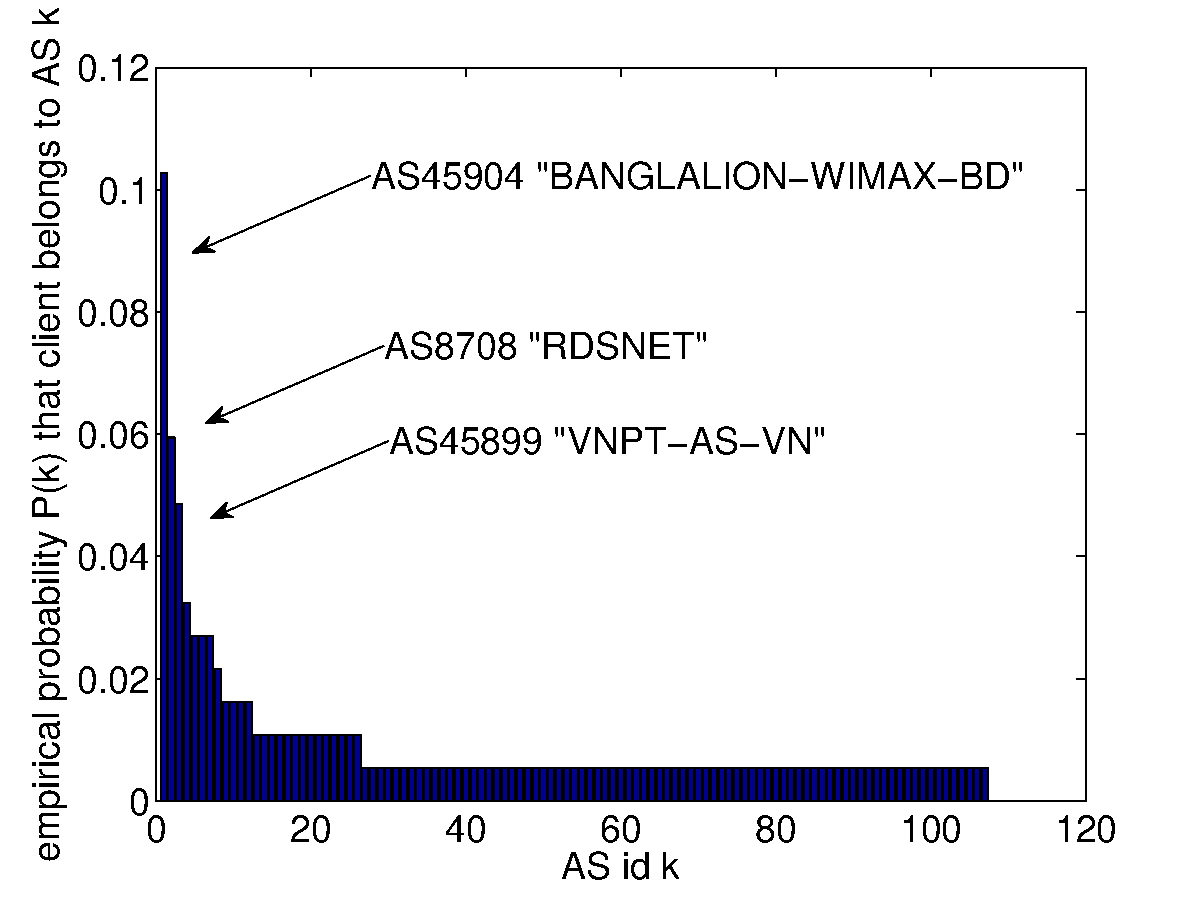
\includegraphics[width=0.5\textwidth]{figures/valli_AS_mw_src.pdf}
%  	\caption{Distribution of crowdsourcing clients over autonomous systems.}
%  	\label{fig:AS_mw_src}
%\end{figure}

%Figure~\ref{fig:AS_pl_dst} shows the autonomous systems of YouTube servers accessed by PlanetLab nodes.
Figure~\ref{fig:AS_dst} shows the autonomous systems of YouTube servers accessed by PlanetLab and Crowdsourcing nodes.
The autonomous systems were ranked by the number of YouTube servers located in the AS.
The empirical probability $P(k)$ that a server belongs to AS with rank $k$ is depicted against the AS rank.
The number of autonomous systems hosting YouTube servers that are accessed by PlanetLab nodes is limited to less than 30.
The top three ranked ASs are AS15169, AS36040 and AS43515.
AS15169 is the Google autonomous system which includes the Google backbone.
The Google backbone is a global network that reaches to worldwide points of presence to offer peering agreements at peering points.
AS36040 is the YouTube network connecting the main datacenter in Mountain-View which is also managed by Google.
AS43515 belongs to the YouTube site in Europe which is administrated in Ireland.
Hence, two thirds of the servers are located in an autonomous systems which is managed by Google.
Only few requests are served from datacenters not being located in a Google AS.
The reason that request from PlanetLab are most frequently served by ASs owned by Google might be a good interconnection of the NRENs to the Google ASs.

% \begin{figure}[bt]
%     \centering
% 	\begin{subfigure}[t]{0.49\textwidth}
% 	\includegraphics[width=\textwidth]{aslevel/crowd/figs/valli_AS_pl_dst.pdf}
%   \caption{PlanetLab}
% 	\label{fig:AS_pl_dst}
%   \end{subfigure}
% 	\begin{subfigure}[t]{0.49\textwidth}
% 	\includegraphics[width=\textwidth]{aslevel/crowd/figs/valli_AS_mw_dst.pdf}
%   \caption{Crowdsourcing}
%  	\label{fig:AS_mw_dst}
%   \end{subfigure}
%     \caption{Distribution of YouTube servers on autonomous systems from a) PlanetLab and b) Crowdsourcing perspective.}
%     \label{fig:AS_dst}
% \end{figure}

\begin{figure}[tb]
	\centering
 	\includegraphics[width=0.7\textwidth]{aslevel/crowd/figs/mwvspllin}
  	\caption{Distribution of YouTube servers on autonomous systems from PlanetLab and Crowdsourcing perspective.}
  	\label{fig:AS_dst}
\end{figure}

%\begin{figure}[tb]
%	\centering
% 	\includegraphics[width=0.5\textwidth]{figures/valli_AS_pl_dst.pdf}
%  	\caption{Distribution of YouTube servers over autonomous systems from PlanetLab perspective.}
%  	\label{fig:AS_pl_src}
%\end{figure}

%Figure~\ref{fig:AS_mw_dst} depicts the autonomous systems where requests to YouTube videos from the crowdsourcing workers were directed.
%The empirical probability that a server belongs to an AS has been plotted dependent on the AS rank.
The YouTube servers identified by the crowdsourcing probes are located in more than 60 autonomous systems.
Hence, the YouTube CDN is expanded on a higher range of ASs from the crowdsourcing perspective compared to PlanetLab.
Again the three autonomous systems serving most requests are the ASs managed by Google, respectively YouTube.
However, the total number of requests served by a Google managed AS is only 41\% as opposed to almost 70\% in the PlanetLab case.
Hence, in contrary to the PlanetLab measurement, requests are served most frequently from ASs not owned by Google.
Here, caches at local ISPs  managed by YouTube could be used to bring the content close to users without providing own infrastructure.
This would also explain the large number of identified ASs providing a YouTube server.
The results show that the PlanetLab platform is not capable to measure the structure of a global CDN, since large parts of the CDN are not accessed by clients in NRENs.
%The aim of this work was to compare the measurement capabilities of the concurring platforms, opposed to a complete measurement of the YouTube CDN.
%It is part of future work to perform an exhaustive measurement study based on PlanetLab and crowdsourcing platforms, which produces a representative view from gobally distributed vantage points on the YouTube CDN and its distribution on autonomous systems.

%Crowdsourcing identifies a higher range of different ASs

%\begin{figure}[tb]
%	\centering
% 	\includegraphics[width=0.5\textwidth]{figures/valli_AS_mw_dst.pdf}
%  	\caption{Distribution of YouTube servers over autonomous systems from crowdsourcing end-user perspective.}
%  	\label{fig:AS_mw_src}
%\end{figure}

%TODO identify overlaps.

%A substantial number of servers is not located in a Google AS
%Heterogeneous distribution. Implication on measurement. Optimize measurement framework?
